\documentclass[11pt,a4paper]{article}

\usepackage{amsmath,amsthm,amssymb}
\usepackage{algorithm}
\usepackage{algpseudocode}
\usepackage{booktabs}
\usepackage{hyperref}
\usepackage{xcolor}
\usepackage{geometry}
\geometry{margin=2.5cm}
\usepackage{graphicx}

% ---------- theorem environments ----------
\newtheorem{theorem}{Theorem}
\newtheorem{lemma}[theorem]{Lemma}
\newtheorem{remark}{Remark}
\newtheorem{definition}{Definition}

% ---------- notation ----------
\newcommand{\RR}{\mathbb{R}}
\newcommand{\eps}{\varepsilon}

% =========================================
\title{Face-Rotation BFS Nets of the Regular and Uniform
  Convex 4-Polytopes}

\author{Takashi Yoshino\thanks{%
  \texttt{tyoshino@toyo.jp}.
  ORCID: 0000-0003-1756-0162.}}

\date{}
% =========================================

\begin{document}
\maketitle

\begin{abstract}
We study the face-rotation BFS unfolding of regular convex 4-poly\-topes:
a breadth-first spanning tree of the cell-adjacency graph is chosen,
and each child cell is rotated about the shared polygonal face into
the parent's 3-dimensional hyperplane.
We prove by exhaustive computational verification that for every one
of the six regular convex 4-polytopes---the 5-cell, 8-cell, 16-cell,
24-cell, 120-cell, and 600-cell---this procedure yields a valid
(non-self-intersecting) 3D net from \emph{every} choice of root cell.
In total, $5+8+16+24+120+600 = 773$ root cells were verified.
This extends the work of Devadoss and Harvey
\cite{DevadossHarvey2022}, who established validity for the 5-, 8-,
and 16-cell for \emph{all} spanning trees and left the remaining three
polytopes open; we resolve the open cases for the BFS subfamily.
By contrast, our result stands in sharp contrast to the apple-peel
unfolding algorithm \cite{YoshinoChaidee2026}, for which the 120-cell
produces no valid nets despite admitting $1{,}440$ valid orderings,
and the 600-cell admits no valid ordering at all.
We also show that regularity is essential: running the same procedure
from all $24{,}487$ roots of the 64 convex uniform 4-polytopes leaves
61 valid from every root, one valid from none, and two valid from some
roots but not others.
\end{abstract}

% =========================================
\section{Introduction}
% =========================================

The question of whether a convex polytope can be \emph{unfolded} into
a non-overlapping flat arrangement of its facets---a \emph{net}---is a
classical problem in discrete geometry, dating back to D\"{u}rer's
depiction of polyhedral nets in the sixteenth century.
In three dimensions the analogous question (does every convex polyhedron
admit a non-overlapping edge unfolding?) remains open as the D\"{u}rer
conjecture \cite{Shephard1975}.
For four-dimensional polytopes, the facets are 3-dimensional cells and
a net is an arrangement of those cells in~$\RR^3$.
Early work on unfolding the 4-cube into 3D arrangements of its cubical
cells was carried out by Turney~\cite{Turney1984}, who enumerated
all 261 topologically distinct nets of the 8-cell (hypercube).

Devadoss and Harvey \cite{DevadossHarvey2022} initiated the systematic
study of ridge unfoldings of the six regular convex 4-polytopes,
proving that every spanning tree of the cell-adjacency graph yields a
valid net for the 4-simplex (5-cell), 4-cube (8-cell), and 4-orthoplex
(16-cell).
They demonstrated failure for the analogous result in dimension $n\ge5$
for orthoplexes, but left the 24-cell, 120-cell, and 600-cell open.

In this paper we study a canonical subfamily of spanning trees,
namely those produced by \emph{breadth-first search} (BFS) from a
chosen root cell, paired with a specific unfolding procedure that we
call \emph{face-rotation}.
Our main result (Theorem~\ref{thm:main}) is that for every regular
convex $4$-polytope and every choice of root cell, this procedure yields
a valid 3D net.
The proof is by exhaustive computational verification.
The result for the 5-, 8-, and 16-cell is a special case of
\cite{DevadossHarvey2022}; the new content is the 24-cell, 120-cell,
and 600-cell.

A companion paper \cite{YoshinoChaidee2026} introduces the
\emph{apple-peel} algorithm, a greedy spiral/zonal ordering of cells
that defines a different family of spanning trees.
That algorithm completes successfully for all $1{,}440$ starting pairs
for the 120-cell, yet every resulting 3D net self-intersects.
For the 600-cell the algorithm cannot even complete the ordering.
The face-rotation BFS algorithm succeeds where apple-peel fails,
illustrating that the existence of a valid ordering and the validity
of a net are independent properties.

This paper is organized as follows.
Section~\ref{sec:theory} recalls the necessary background and describes
the face-rotation BFS algorithm.
Section~\ref{sec:results} states and verifies Theorem~\ref{thm:main}
and discusses the contrast with apple-peel unfolding.
Section~\ref{sec:uniform} runs the same procedure over the 64 convex
uniform 4-polytopes and shows that the theorem does not survive the
loss of regularity.
Section~\ref{sec:open} collects open problems.

% =========================================
\section{Preliminaries}\label{sec:theory}
% =========================================

\subsection{Background}\label{sec:background}

%\subsection{Regular convex 4-polytopes}

There are exactly six regular convex 4-polytopes (see
Coxeter~\cite{Coxeter1973}).
Their Schl\"{a}fli symbols and combinatorial data are listed in
Table~\ref{tab:polytopes}.

\begin{table}[ht]
\centering
\caption{The six regular convex 4-polytopes.}
\label{tab:polytopes}
\begin{tabular}{lcccccc}
\toprule
Polytope & Symbol & Vertices & Faces & Cells & Cell type & Cell degree\\
\midrule
5-cell    & $\{3,3,3\}$ &   5 &   10 &    5 & tetrahedron    & 4 \\
8-cell    & $\{4,3,3\}$ &  16 &   24 &    8 & cube           & 6 \\
16-cell   & $\{3,3,4\}$ &   8 &   32 &   16 & tetrahedron    & 4 \\
24-cell   & $\{3,4,3\}$ &  24 &   96 &   24 & octahedron     & 8 \\
120-cell  & $\{5,3,3\}$ & 600 &  720 &  120 & dodecahedron   & 12\\
600-cell  & $\{3,3,5\}$ & 120 & 1200 &  600 & tetrahedron    & 4 \\
\bottomrule
\end{tabular}
\end{table}

\noindent
Here \emph{cell degree} denotes the number of cells adjacent to each
cell (sharing a ridge, i.e., a 2-face).

%\subsection{Ridge unfoldings}

Following Devadoss and Harvey \cite{DevadossHarvey2022}, a \emph{ridge unfolding} of a
4-polytope $P$ is specified by a spanning tree $T$ of the
cell-adjacency graph $G(P)$ (nodes = cells, edges = shared
ridges, i.e., shared $2$-faces).
The unfolding is performed inductively: a root cell is placed in some
3D hyperplane $H$; for each edge $(p, c)$ in $T$ directed away from
the root, the child cell $c$ is rigidly rotated about the
shared polygon with its parent $p$ until it lies in the same
hyperplane as $p$.
The resulting arrangement is a \emph{net} if no two cells overlap in
their interiors.

Ridge unfoldings are also accessible through interactive software.
Stella4D~\cite{Webb2026} has displayed 3D nets of polychora since
2007 and lets the user reglue cells one at a time, so that in
principle any spanning tree can be realized by hand.
Its nets are generated to maximize symmetry and visual appeal rather
than to realize a prescribed family of spanning trees, and, as its
documentation states, intersections between cells are ignored.
Whether an unfolding is free of self-intersection---the question
studied here---is therefore outside the scope of such tools.

\begin{definition}[BFS spanning tree]\label{def:bfs}
Let $G(P)$ be the cell-adjacency graph of a 4-polytope $P$ and let
$r$ be a root cell.
The \emph{BFS spanning tree} of $G(P)$ rooted at $r$ is the spanning
tree $T$ obtained by breadth-first traversal from $r$: cells are
discovered layer by layer, and each newly encountered cell is connected
to the cell from which it was first reached.
When multiple neighbors of the current frontier are simultaneously
eligible, their relative order is determined by a fixed
\emph{tie-breaking rule}; different rules may yield different trees.
\end{definition}

% =========================================
\subsection{Face-Rotation BFS Algorithm}\label{sec:algorithm}
% =========================================

%\subsection{Algorithm description}

Given a 4-polytope $P$ with vertex set $V\subset\RR^4$,
cell set $C$, and a root cell $r\in C$, the algorithm proceeds
as follows.

\paragraph{Step 1: Face-up rotation.}
Let $\bar{V} = \{v - \bar{v} : v\in V\}$ where $\bar{v}$ is the
centroid of $V$.
Let $c_r = \mathrm{centroid}(\{v\in \bar{V}: v\text{ is a vertex of }r\})$.
Apply the rotation $R\in\mathrm{SO}(4)$ that maps
$c_r/\|c_r\|$ to the unit vector $\hat{w} = (0,0,0,1)$.
(If $c_r/\|c_r\| = \hat{w}$ we take $R=I$; if $c_r/\|c_r\|=-\hat{w}$
we negate all coordinates.)
This \emph{face-up} rotation ensures that the root cell's centroid
lies on the positive $w$-axis, making subsequent unfolding into the
hyperplane $\{w=\mathrm{const}\}$ numerically stable.

\paragraph{Step 2: BFS traversal.}
Maintain a FIFO queue $Q$ initialized with the root cell $r$,
and a visited set $\mathrm{Vis} = \{r\}$ with $T_r = \mathrm{id}$.
While $Q$ is non-empty, dequeue the front cell $p$;
for each neighbor $c$ of $p$ in $G(P)$, taken in the order they
appear in the adjacency list, if $c \notin \mathrm{Vis}$: add $c$ to $\mathrm{Vis}$,
enqueue $c$, and compute the cumulative 4D affine transform $T_c$
by the procedure in Algorithm~\ref{alg:unfoldTF}.
The algorithm terminates when $Q$ is empty (no candidates remain);
since $G(P)$ is connected for every regular 4-polytope,
all cells are visited.
The order in which neighbors are added to $Q$ constitutes the
tie-breaking rule of Definition~\ref{def:bfs} and determines which
BFS spanning tree is produced.
In our implementation, ties are broken by the order in which neighbors
appear in the adjacency list of the input data.

\paragraph{Step 3: Projection.}
Apply each $T_c$ to the vertices of cell $c$, obtaining
$\{\,T_c(v)\in\RR^4 : v \in c\,\}$.
After Step~2, the $w$-coordinate of every transformed vertex satisfies
$|w - w_0| \le \eps_w$ for a common value $w_0$ and numerical
tolerance $\eps_w \approx 10^{-13}$.
Discard the $w$-coordinate; the resulting $(x,y,z)$-coordinates form
the 3D net.

\begin{algorithm}[ht]
\caption{\textsc{UnfoldTransform}$(p, c, T_p)$}
\label{alg:unfoldTF}
\begin{algorithmic}[1]
\Require parent cell $p$ with cumulative transform $T_p$; child cell $c$
\Ensure cumulative transform $T_c$ for $c$
\State Let $f_1,\ldots,f_k$ be the vertices of the shared face of $p$ and $c$
       (in the original 4D frame)
\State $\tilde{f}_i \leftarrow T_p(f_i)$ for all $i$
       \Comment{shared face in parent's unfolded frame}
\State $c_f \leftarrow \frac{1}{k}\sum_i \tilde{f}_i$
       \Comment{face centroid}
\State Compute orthonormal basis $\{u_1, u_2\}$ of the face plane via
       Gram-Schmidt on $\{\tilde{f}_i - c_f\}$
\State $n_p \leftarrow \text{component of }(T_p(\mathrm{centroid}(p)) - c_f)
       \text{ orthogonal to } \{u_1,u_2\}$, normalized
\State $n_c \leftarrow \text{component of }(T_p(\mathrm{centroid}(c)) - c_f)
       \text{ orthogonal to } \{u_1,u_2\}$, normalized
\State $\theta \leftarrow \arccos\!\bigl(\max(-1,\,\min(1,\,n_c\cdot(-n_p)))\bigr)$
\State $e_1 \leftarrow n_c$; \;
       $e_2 \leftarrow \mathrm{normalize}(-n_p - (n_c\cdot(-n_p))\,n_c)$
       \Comment{if degenerate, use any vector $\perp\{u_1,u_2,n_c\}$}
\State $R \leftarrow I_4 + (\cos\theta-1)(e_1 e_1^\top + e_2 e_2^\top)
       + \sin\theta(e_2 e_1^\top - e_1 e_2^\top)$
       \Comment{4D rotation in the plane $\{e_1,e_2\}$}
\State \Return $\bigl(R,\; c_f - R\,c_f\bigr)\circ T_p$
       \Comment{compose affine maps}
\end{algorithmic}
\end{algorithm}

%\subsection{Intersection test}

A naive implementation using \emph{closed-region} membership
(e.g.\ Mathematica's \texttt{RegionMember}) incorrectly classifies
cells as overlapping when they share only a face, edge, or vertex
in the net.
This is particularly acute for pointed cells such as tetrahedra and
octahedra, which frequently share edges and vertices with
cells not connected by a tree edge.

We use the following \emph{volume-based} test, which detects only
interior overlaps.

\begin{remark}
Two cells not connected by an edge of $T$ may share a face, edge,
or vertex in the unfolded net without overlapping in their interiors.
A correct validity test must detect only \emph{interior} overlaps.
\end{remark}

\begin{definition}[Valid net]\label{def:valid}
A net is \emph{valid} if for every pair of cells $(i,j)$ not
connected by an edge of $T$,
\[
  \mathrm{Vol}_3\!\bigl(\mathrm{conv}(c_i)\cap\mathrm{conv}(c_j)\bigr)
  \;\le\; \eps_{\mathrm{vol}}
\]
where $\mathrm{conv}(c_i)$ denotes the convex hull of cell $i$'s
vertices in 3D, and $\eps_{\mathrm{vol}} = 10^{-8}$.
\end{definition}

\noindent
In practice we first apply a bounding-box filter to exclude pairs
that clearly cannot overlap, then compute
\texttt{RegionMeasure[\allowbreak RegionIntersection[$h_i$, $h_j$]]}
in Mathematica for the remaining candidate pairs,
where $h_i$ denotes the convex hull mesh of cell $i$'s vertices in 3D.

\begin{remark}
Using closed-region membership instead of volume intersection would
report the 16-cell, 24-cell, and 600-cell as invalid (false positives
due to boundary contact), contradicting the correct result.
The volume threshold $\eps_{\mathrm{vol}} = 10^{-8}$ is
well below the smallest possible cell volume (even for the 600-cell,
where each tetrahedral cell has volume $\approx 3\times10^{-3}$
at the scale used), so no true interior overlap is missed.
\end{remark}

% =========================================
\section{Results}\label{sec:results}
% =========================================

\subsection{Main result}

\begin{theorem}[Main]\label{thm:main}
For every regular convex $4$-polytope~$P$ and every cell $r\in P$,
a face-rotation BFS net of $P$ rooted at $r$ is valid.
\end{theorem}

\begin{proof}
Exhaustive computational verification.
For each of the six polytopes we loaded the combinatorial data
(vertices, faces, cells) from the data files available in the repository,
ran the face-rotation BFS algorithm for every root cell,
and applied the volume-based intersection test
(Definition~\ref{def:valid}) to every pair of cells not connected
by a tree edge.
Table~\ref{tab:contrast} summarizes the results, and
Figure~\ref{fig:allnets} shows representative nets for each polytope.
The $w$-coordinate spread after unfolding was at most $4\times10^{-13}$
in all cases, confirming that all cells lie in a common 3D hyperplane
to numerical precision.
\end{proof}

\begin{table}[ht]
\centering
\caption{Comparison of face-rotation BFS and apple-peel RZ unfolding.
  ``Valid orderings'' = fraction of $(C_1, C_2)$ pairs for which
  apple-peel visits all cells;
  ``Valid nets'' = fraction of valid orderings that produce a
  non-self-intersecting 3D net.}
\label{tab:contrast}
\begin{tabular}{lcccc}
\toprule
& & \multicolumn{1}{c}{Face-rotation BFS}
  & \multicolumn{2}{c}{Apple-peel RZ \cite{YoshinoChaidee2026}} \\
\cmidrule(lr){3-3}\cmidrule(lr){4-5}
Polytope & Cells & Valid (all roots) & Valid orderings & Valid nets \\
\midrule
5-cell   &    5 &   5/5   & 20/20 (100\%)     & 20/20 (100\%)         \\
8-cell   &    8 &   8/8   & 48/48 (100\%)     & 48/48 (100\%)         \\
16-cell  &   16 &  16/16  & 20/64 (31\%)      & 20/20 (100\%)         \\
24-cell  &   24 &  24/24  & 192/192 (100\%)   & 192/192 (100\%)       \\
120-cell &  120 & 120/120 & 1440/1440 (100\%) & \textbf{0/1440 (0\%)} \\
600-cell &  600 & 600/600 & \textbf{0/2400 (0\%)} & ---               \\
\bottomrule
\end{tabular}
\end{table}

\begin{remark}
For the 5-, 8-, and 16-cell, Theorem~\ref{thm:main} is a special
case of the stronger result of Devadoss and Harvey
\cite{DevadossHarvey2022}, who proved that \emph{all} spanning trees
of the cell-adjacency graph (not just BFS trees) yield valid nets.
The new content of Theorem~\ref{thm:main} is therefore the 24-cell,
120-cell, and 600-cell.
\end{remark}

\begin{remark}[On the number of verifications]\label{rem:equivariance}
Each regular convex $4$-polytope has a symmetry group acting
transitively on cells.
If the BFS algorithm uses a geometrically equivariant tie-breaking
rule, then for any symmetry $g$ mapping root $r$ to root $r'$,
the net from $r'$ is the image of the net from $r$ under $g$,
and validity is preserved by the rigidity of $g$.
In that case, verification of a \emph{single} root cell per polytope
would suffice to establish Theorem~\ref{thm:main}.
Our implementation uses index-based tie-breaking in the BFS queue,
which is not equivariant under the symmetry group; we therefore
verified all $773$ roots independently.
In either case, Theorem~\ref{thm:main} guarantees the
\emph{existence} of a valid face-rotation BFS net from every root cell
under this tie-breaking rule.
Whether validity holds for every possible tie-breaking rule remains open.
\end{remark}

\begin{figure}[p]
  \centering
  \includegraphics[width=\textwidth]{260612AllFaceRotation.pdf}
  \caption{Face-rotation BFS nets of the six regular convex 4-polytopes.
    Top row (left to right): 5-cell, 8-cell, 16-cell, 24-cell.
    Bottom row: 120-cell, 600-cell.
    Shading indicates BFS layer depth (dark\,=\,root cell, light\,=\,periphery).
    STL files of all six nets are available in the repository (see Code and Data Availability).}
  \label{fig:allnets}
\end{figure}

% =========================================
\subsection{Contrast with Apple-Peel Unfolding}\label{sec:contrast}
% =========================================

The apple-peel algorithm \cite{YoshinoChaidee2026} constructs a
spanning tree by greedily selecting the next cell according to a
global spiral (RS) or zonal (RZ) criterion, without the layer-by-layer
structure of BFS.
Table~\ref{tab:contrast} compares the two algorithms.

\noindent
The most striking contrast occurs for the 120-cell and 600-cell:

\begin{itemize}
\item \textbf{120-cell}: Apple-peel produces $1{,}440$ valid orderings
  (all $(C_1, C_2)$ pairs succeed), yet every resulting 3D net
  self-intersects~\cite{YoshinoChaidee2026}.
  Face-rotation BFS yields a valid net from every root.

\item \textbf{600-cell}: Apple-peel cannot complete any ordering
  (structural impossibility due to the 4-regular cell-adjacency graph).
  Face-rotation BFS yields a valid net from every root.
\end{itemize}

These cases demonstrate that \emph{the existence of a valid ordering
and the validity of the resulting 3D net are independent properties}.
A spanning tree that is well-suited for the ordering problem
need not yield a geometrically valid net, and vice versa.

% =========================================
\section{The Uniform Case}\label{sec:uniform}
% =========================================

Theorem~\ref{thm:main} does not extend to the convex uniform
4-polytopes.
Excluding the two infinite prismatic families, there are exactly 64 of
these; unlike the enumeration of all uniform 4-polytopes, which is
still open, this list is known to be complete, the exceptional
non-Wythoffian member being the grand antiprism of Conway and
Guy~\cite{ConwayGuy1965}.
We generated all 64 and ran the face-rotation BFS unfolding from every
cell, $24{,}487$ roots in all.

\paragraph{Construction.}
The 45 distinct Wythoffian members of the $A_4$, $B_4$, $F_4$ and
$H_4$ families were built from their Coxeter diagrams: the group is
generated as the closure of the four mirror reflections, the vertices
are the orbit of the point whose distance to each ringed mirror
is~$1$ and to each unringed mirror~$0$ (the edge generated by mirror
$i$ has length twice that distance, so equal distances force equal
edge lengths), and the $d$-faces are the orbits of the rank-$d$
parabolic subgroups.
The snub 24-cell and the grand antiprism are not Wythoffian in this
sense, but both arise as diminishings of the 600-cell: delete an
inscribed 24-cell, respectively two orthogonal decagonal rings, and
take the convex hull.
In each case the surviving cells are the 600-cell tetrahedra avoiding
every deleted vertex, together with one cell per deleted vertex,
namely the hull of its remaining neighbors.
The 17 prisms are the prisms over the 5 Platonic and 13 Archimedean
solids, with lateral edge length equal to the edge length of the base,
minus the cube prism, which is the tesseract and already regular.
Each construction was checked against the group-theoretic predictions
for the vertex and cell counts, the Euler relation
$V-E+F-C=0$, the requirement that every ridge lie in exactly two
cells, and vertex-transitivity of the vertex degree.

\paragraph{Results.}
The outcome splits three ways, as summarized in
Table~\ref{tab:uniform}.

\begin{table}[ht]
\centering
\caption{Face-rotation BFS nets of the 64 convex uniform 4-polytopes,
  over all root cells.}
\label{tab:uniform}
\begin{tabular}{lrrrrr}
\toprule
Family & Polytopes & Roots & All valid & Root-dependent & None valid\\
\midrule
$A_4$, $B_4$, $F_4$   & 30 & $1{,}893$  & 29 & 0 & 1\\
$H_4$                 & 15 & $21{,}600$ & 13 & 2 & 0\\
Snub 24-cell, grand antiprism & 2 & 464 & 2 & 0 & 0\\
Prisms                & 17 & 530        & 17 & 0 & 0\\
\midrule
Total                 & 64 & $24{,}487$ & 61 & 2 & 1\\
\bottomrule
\end{tabular}
\end{table}

\noindent
Sixty-one of the 64 yield a valid net from every root.
The runcinated 24-cell $t_{0,3}\{3,4,3\}$ yields one from no root: all
240 of its unfoldings self-intersect, in between 3 and 23 pairs of
cells.
The remaining two are \emph{root-dependent}: the runcitruncated
600-cell $t_{0,2,3}\{5,3,3\}$ succeeds from 47 of its $2{,}640$ roots
and the runcitruncated 120-cell $t_{0,1,3}\{5,3,3\}$ from $2{,}570$
of $2{,}640$.
Figure~\ref{fig:uniformfail} shows one failure of each kind.

\begin{figure}[ht]
\centering
\begin{minipage}[b]{0.47\textwidth}
  \centering
  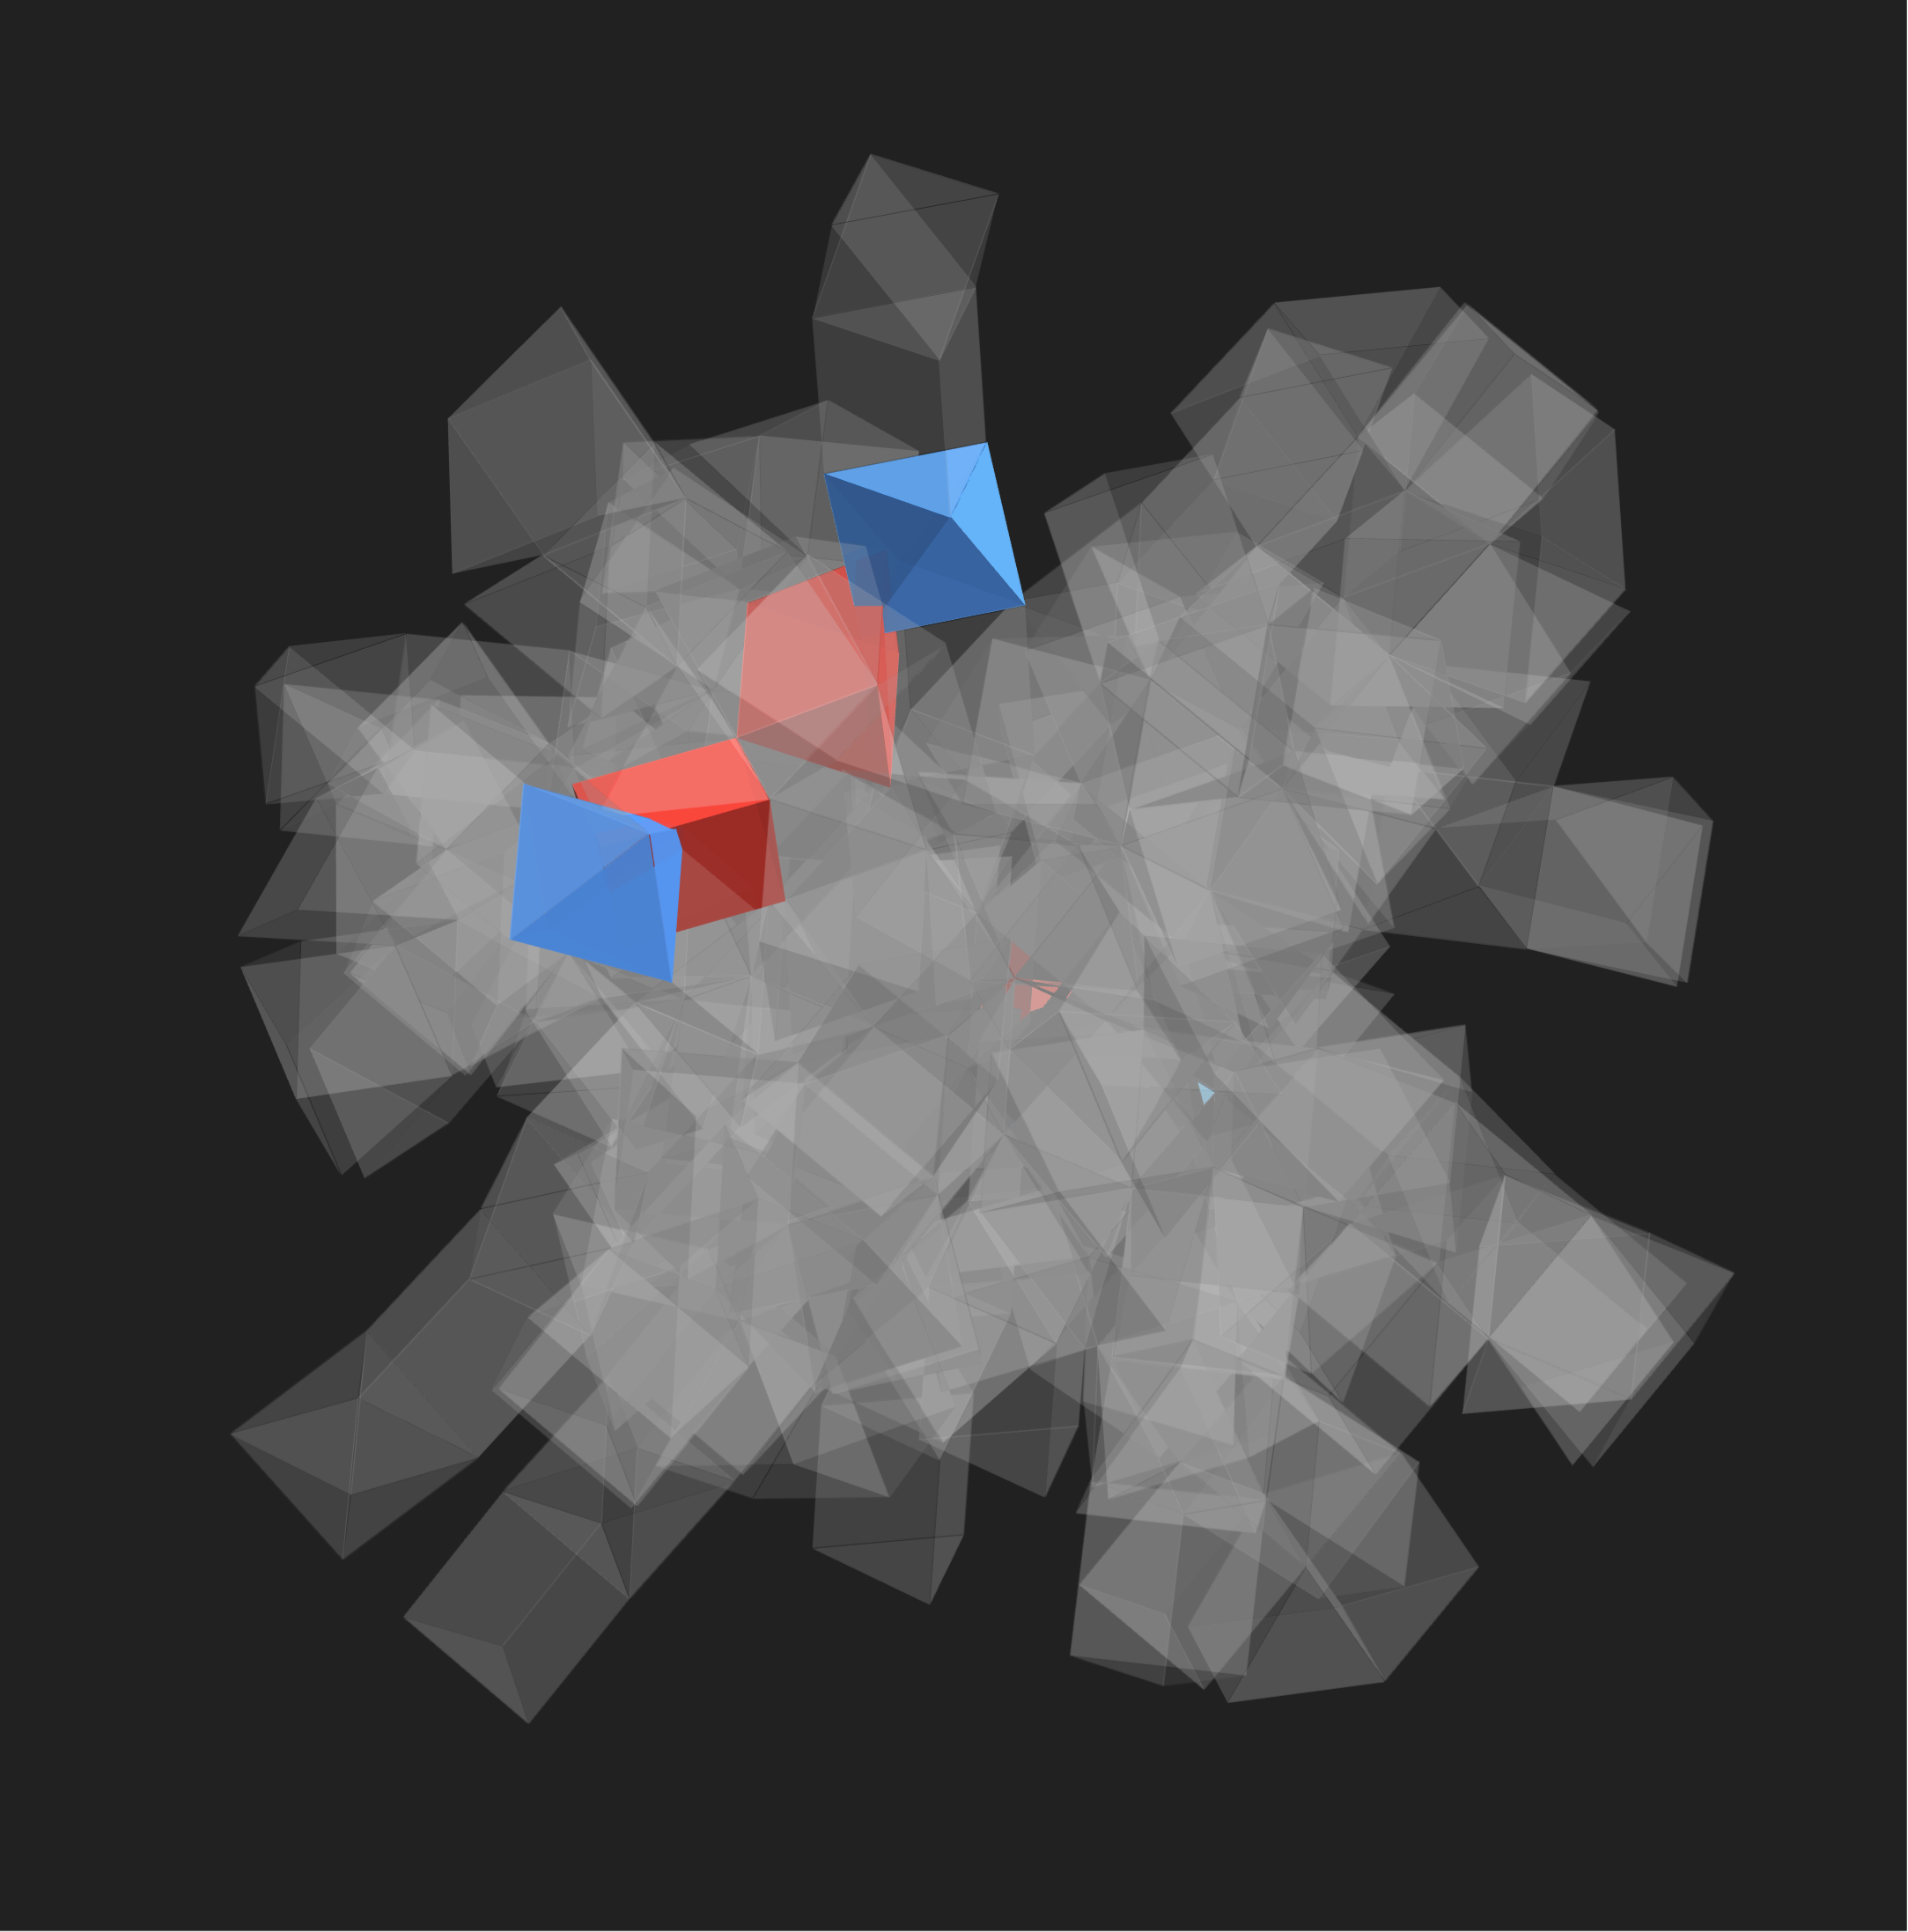
\includegraphics[width=\textwidth]{fig_uniform_a_black.png}\\[2pt]
  {\small (a)}
\end{minipage}\hfill
\begin{minipage}[b]{0.47\textwidth}
  \centering
  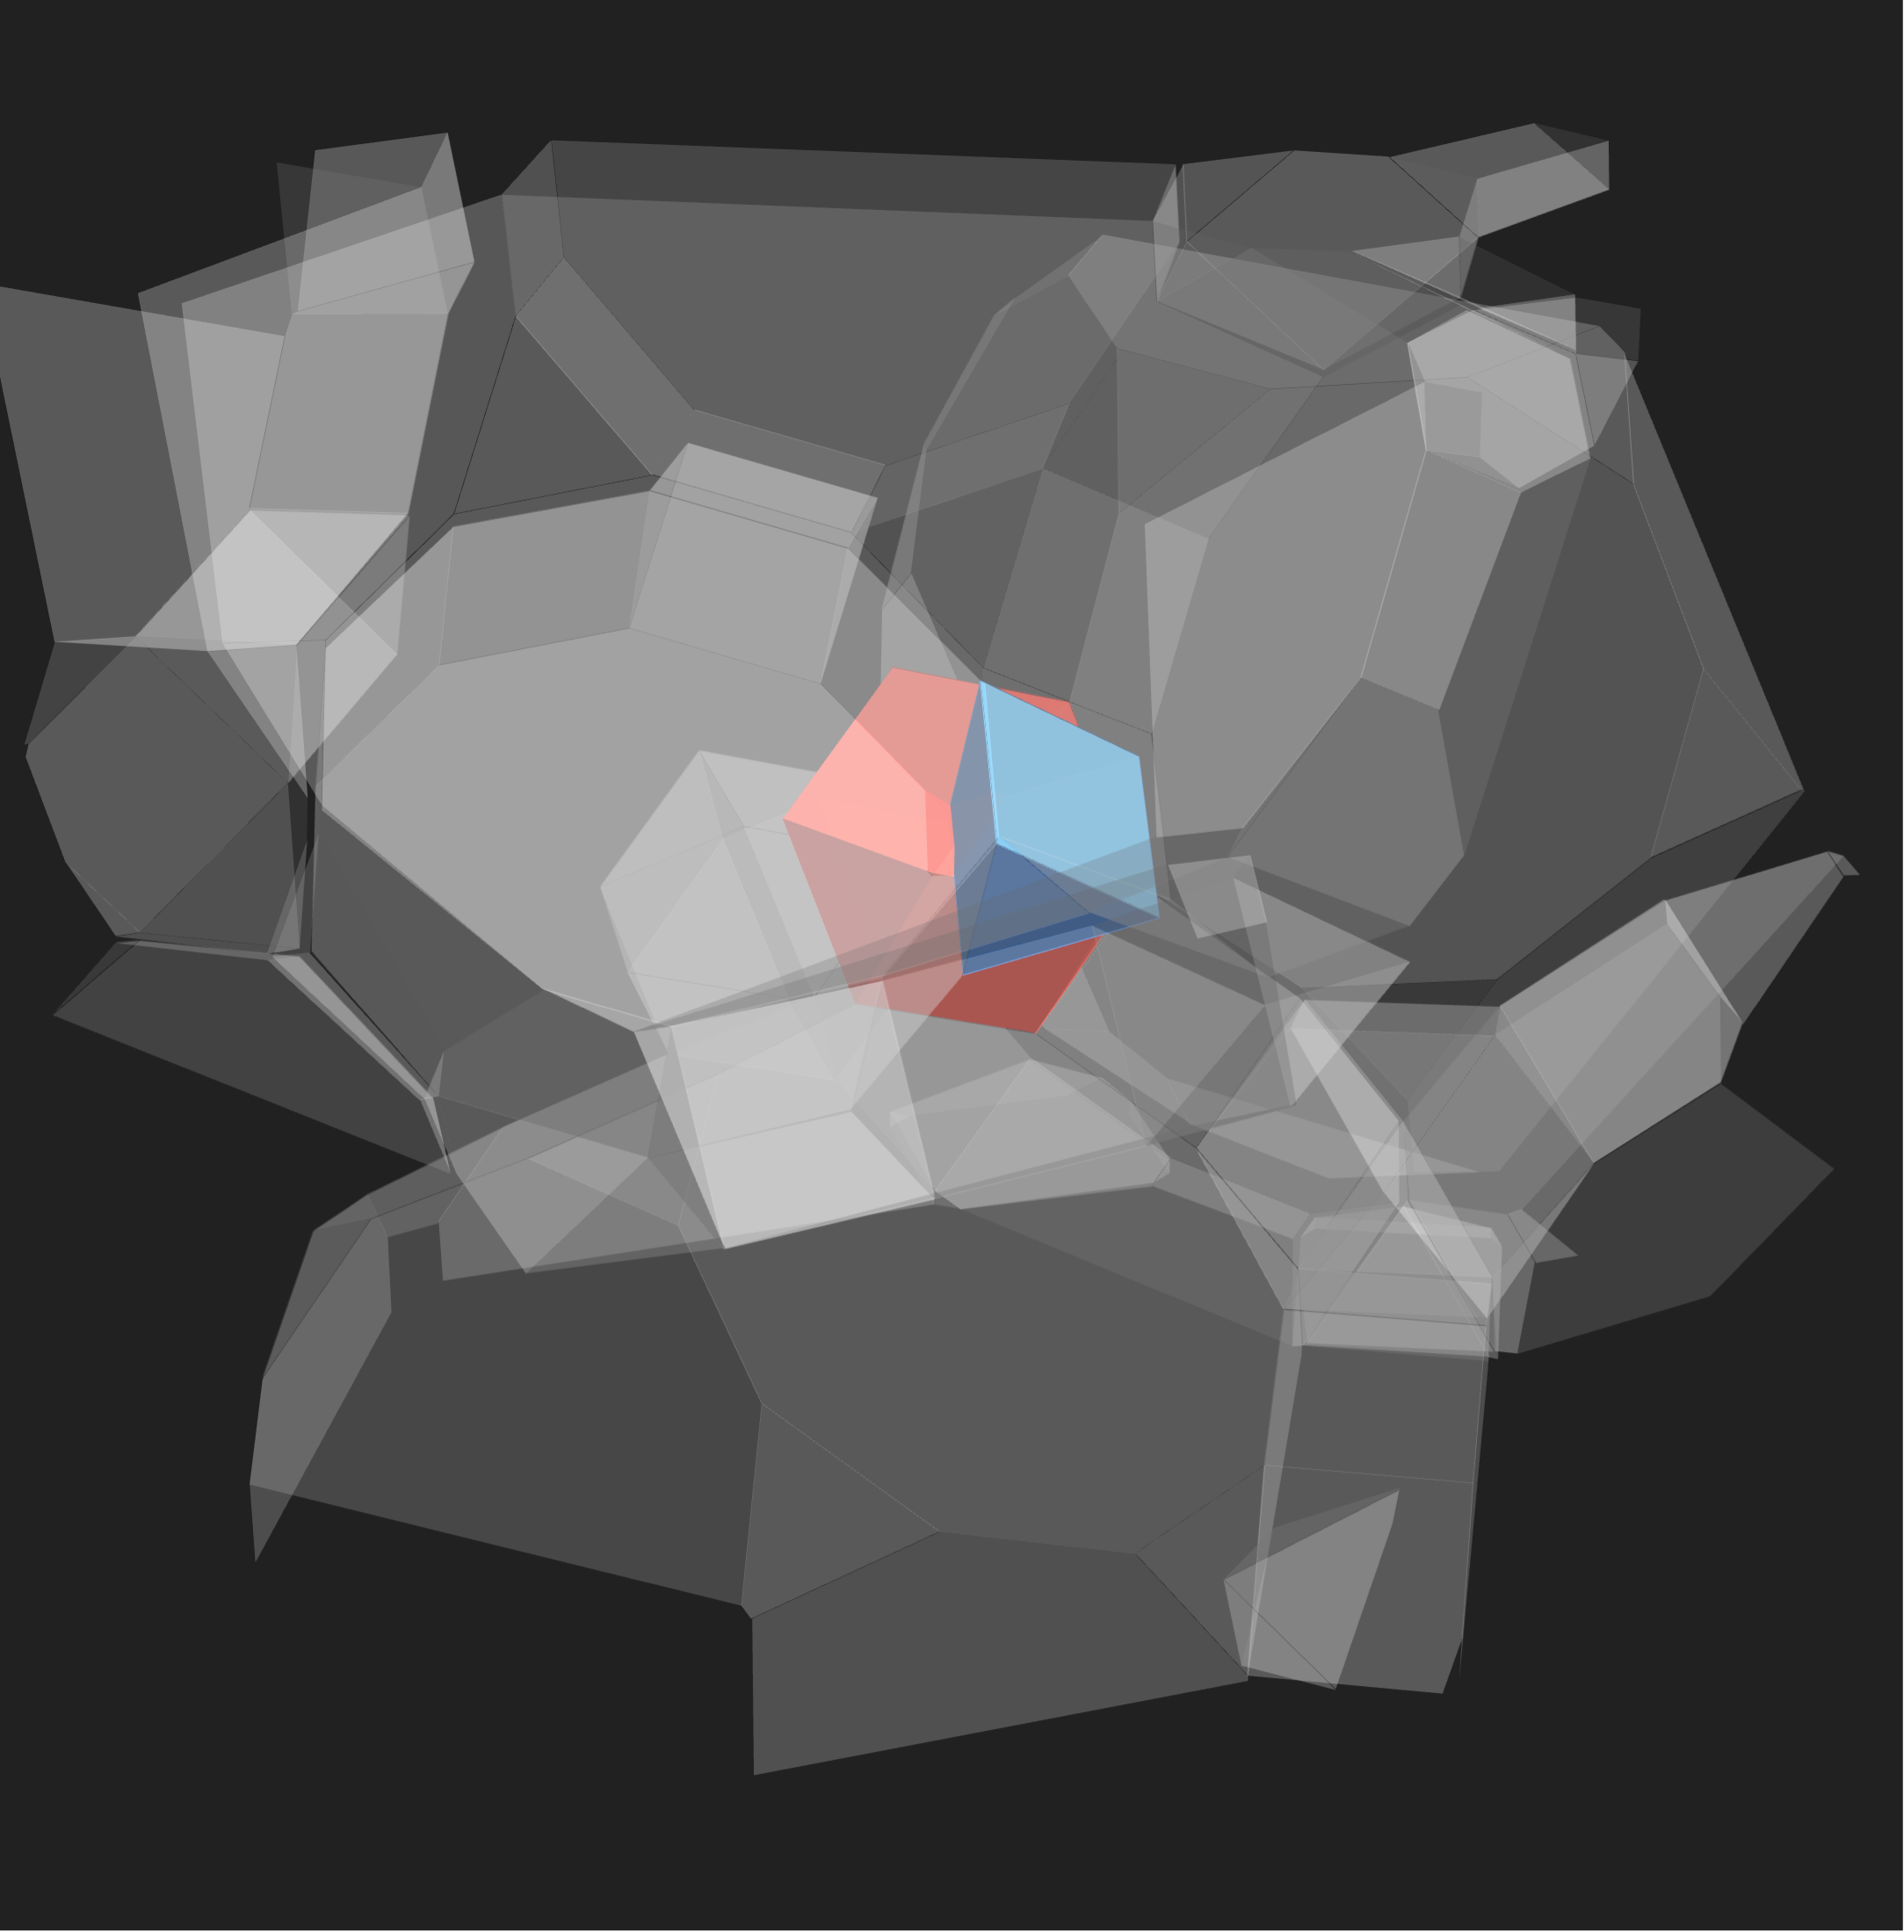
\includegraphics[width=\textwidth]{fig_uniform_b_black.png}\\[2pt]
  {\small (b)}
\end{minipage}
\caption{The two ways the unfolding fails.
  The panels are at deliberately different scales, because the claims
  they carry are about different things: (a) is about a polytope,
  (b) about a single root.
  (a) The runcinated 24-cell at its \emph{best} root, drawn whole:
  3 of its 240 cells intersect a partner, the fewest over all 240
  roots, and no root does better than 3.
  (b) The runcitruncated 120-cell at one of its 70 failing roots,
  drawn as a close-up of the single intersecting pair together with
  its neighbors; the other $2{,}570$ roots are fine.
  In both panels the two members of an intersecting pair are drawn in
  different colors.}
\label{fig:uniformfail}
\end{figure}

The two root-dependent cases are the informative ones.
For every regular 4-polytope the choice of root is immaterial, and it
is tempting to read that as a consequence of cell-transitivity.
The uniform case shows that once cell-transitivity is dropped,
validity genuinely depends on where the unfolding starts: admitting
\emph{some} valid face-rotation BFS net and admitting one from
\emph{every} root are different properties, and
Theorem~\ref{thm:main} establishes the stronger one only in the
regular case.

Cell degree does not separate the three outcomes, in either direction.
The grand antiprism and the snub 24-cell both contain cells of
degree~4---the same poverty of connection that makes the 600-cell
impossible for apple-peel unfolding---yet both are valid from every
root, while the runcinated 24-cell has minimum cell degree~5 and is
valid from none.
Nor does high degree help: every prism has two cells adjacent to all
of the others, up to degree~92 for the prism over the snub
dodecahedron, and all 17 are valid from every root, whereas the
root-dependent runcitruncated 120-cell also carries cells of
degree~32.

\paragraph{Caveats.}
The BFS tree depends on the tie-breaking rule of
Definition~\ref{def:bfs}.
For a cell-transitive polytope the rule is immaterial, but the uniform
polytopes have several cell orbits, so the counts $47$ and $2{,}570$
above are those of one fixed rule (cell index order); another rule may
change them.
For the polytopes with more than a few hundred cells the intersection
test was carried out with a separating-axis implementation rather than
by measuring the volume of the intersection; the two were checked to
return identical verdicts, and identical numbers of intersecting
pairs, on every one of the $1{,}893$ roots of the 30 polytopes of the
$A_4$, $B_4$ and $F_4$ families, and again on a sample of roots of the
two root-dependent cases, where the verdict is also stable as the
separation tolerance ranges over $10^{-4}$ to $10^{-10}$.

% =========================================
\section{Open Problems}\label{sec:open}
% =========================================

The main open question raised by this work is:

\begin{quote}
\textit{Why does face-rotation BFS always produce a valid net for
regular 4-polytopes?
Is there a theoretical proof that does not rely on computer
enumeration?}
\end{quote}

A second open problem is whether Theorem~\ref{thm:main} extends to
all spanning trees (not just BFS) for the 24-cell, 120-cell, and
600-cell, as was proved for the 5-, 8-, and 16-cell by
\cite{DevadossHarvey2022}.

A third question is the characterization left open by
Section~\ref{sec:uniform}.
What distinguishes the 61 uniform 4-polytopes that unfold from every
root, from the two that unfold from some roots only, and from the
runcinated 24-cell, which unfolds from none?
As noted there, cell degree does not decide it, and we have no
candidate invariant that does.
A related question is how far the counts for the two root-dependent
cases depend on the tie-breaking rule: whether some rule makes them
valid from every root, or whether root-dependence survives every
choice.

Finally, extensions to higher dimensions are open as well.

% =========================================
\section*{Code and Data Availability}
% =========================================

All Mathematica scripts implementing the face-rotation BFS algorithm,
the volume-based intersection test, and the visualization are available
at \url{https://github.com/takashi-randomwalker/apple-peel-4d}.
The same repository contains the constructions used for
Section~\ref{sec:uniform}---the Wythoff generator, the two
diminishings of the 600-cell, and the prisms---and the
separating-axis implementation of the intersection test used for the
larger polytopes, together with its agreement check against the
volume-based test.
It also contains the combinatorial data of all 64 convex uniform
4-polytopes, the nets exported as STL and OFF, and the verdict for
each of the $24{,}487$ individual roots.
STL files of the face-rotation BFS nets for all six polytopes (root cell~1)
are also provided in the same repository.

% =========================================
\section*{Acknowledgements}
% =========================================

The author declares no known competing financial interests or personal
relationships that could have appeared to influence the work reported
in this paper.

% =========================================
\begin{thebibliography}{10}

\bibitem{Coxeter1973}
H.~S.~M. Coxeter.
\newblock {\em Regular Polytopes}.
\newblock Dover Publications, 3rd edition, 1973.

\bibitem{ConwayGuy1965}
J.~H. Conway and M.~J.~T. Guy.
\newblock Four-dimensional Archimedean polytopes.
\newblock In {\em Proceedings of the Colloquium on Convexity},
  pages 38--39, Copenhagen, 1965.

\bibitem{DevadossHarvey2022}
S.~L. Devadoss and M.~S. Harvey.
\newblock Unfoldings and nets of regular polytopes.
\newblock {\em Computational Geometry: Theory and Applications},
  111:\penalty0 101977, 2023.
\newblock \href{https://arxiv.org/abs/2111.01359}{arXiv:2111.01359}.

\bibitem{Shephard1975}
G.~C. Shephard.
\newblock Convex polytopes with convex nets.
\newblock {\em Mathematical Proceedings of the Cambridge Philosophical
  Society}, 78(3):389--403, 1975.

\bibitem{Turney1984}
P.~D. Turney.
\newblock Unfolding the tesseract.
\newblock {\em Journal of Recreational Mathematics}, 17(1):1--16, 1984.

\bibitem{Webb2026}
R.~Webb.
\newblock {\em Stella4D: Polyhedron Navigator}, version 6.0.
\newblock Software3D, 2026.
\newblock \href{https://www.software3d.com/Stella.php}
  {https://www.software3d.com/Stella.php}.

\bibitem{YoshinoChaidee2026}
T.~Yoshino and S.~Chaidee.
\newblock Apple-peel unfolding in three and four dimensions:
  Spiral and zonal selection rules.
\newblock {\em arXiv:2605.30373}, 2026.

\end{thebibliography}

\end{document}
